\glspl{uav}, commonly referred to as drones, have become an essential tool across a wide range of applications, including surveying, inspection, and research. Their ability to operate in confined or inaccessible environments makes them particularly valuable for close-range observation and monitoring tasks. Unlike outdoor drones that rely on satellite-based positioning systems such as GPS, indoor drones must depend entirely on onboard sensing, control algorithms, and communication systems to maintain stability and navigate safely. Operating in enclosed environments presents additional challenges, including limited spatial awareness, airflow disturbances, and heightened safety risks due to proximity to structures and personnel. Consequently, the design of an indoor drone requires careful consideration of system architecture, control robustness, and physical safety features. 

\begin{figure}[H]
    \centering
    \captionsetup{justification=centering, margin=1cm}
    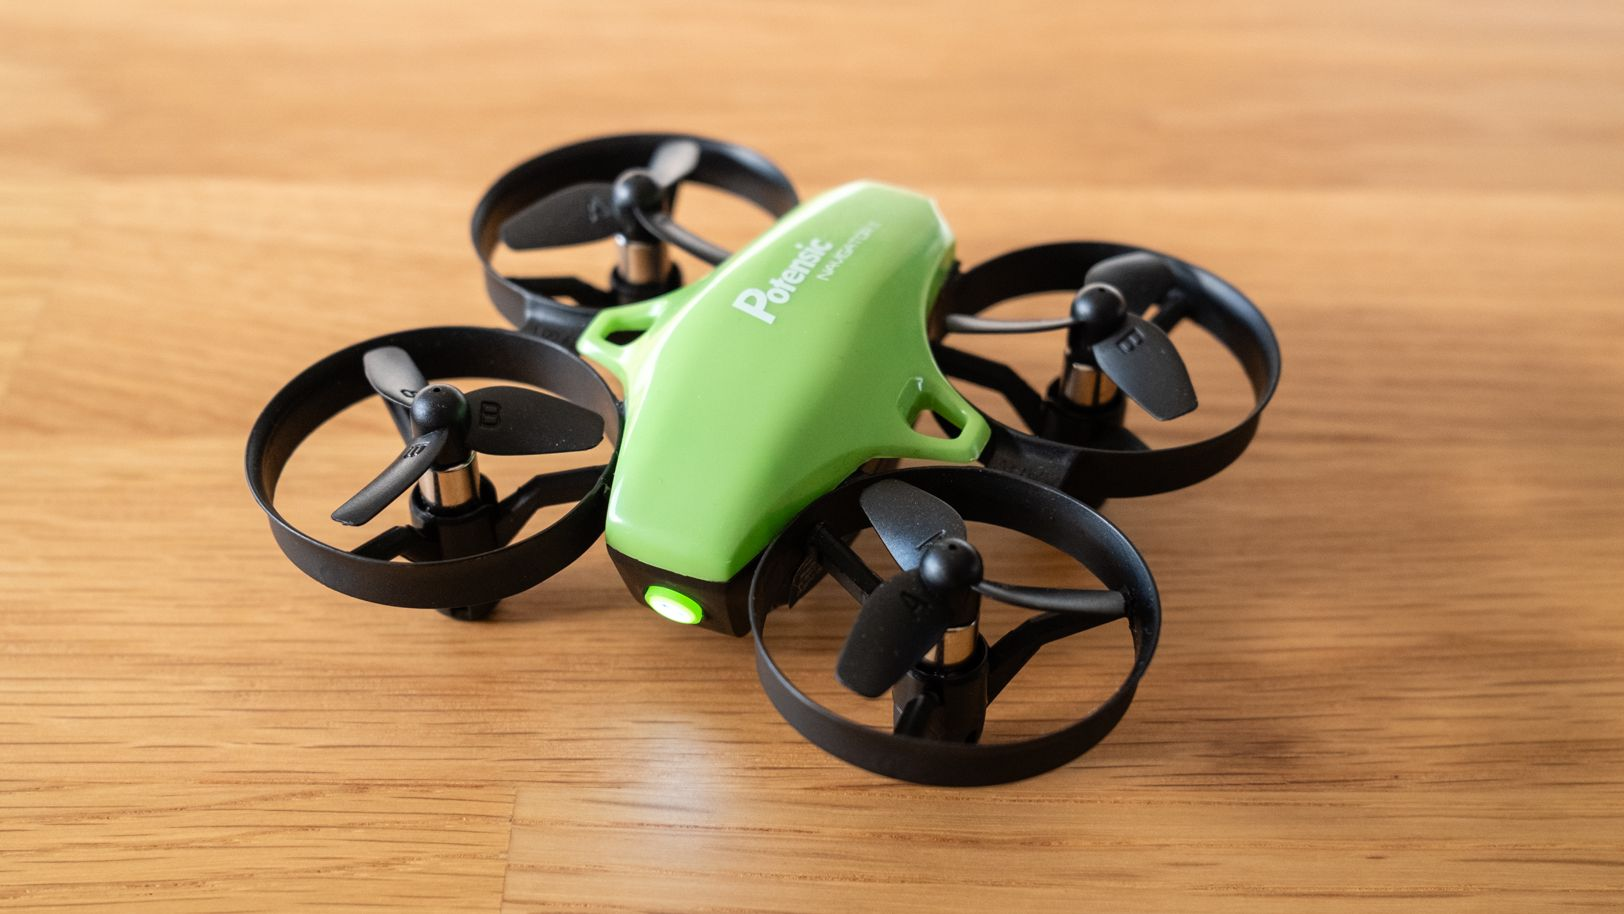
\includegraphics[width=0.4\textwidth]{img/mini-drone.JPG}
    \caption{Miniature Drone \cite{abbott2024}}
\end{figure}

The \gls{uwaal} has commissioned the development of an indoor drone system capable of autonomous and stable flight within a confined environment. The drone will be used to survey and inspect indoor areas such as garages or laboratory spaces, following predefined flight paths and maintaining stable altitude and position despite the influence of external airflow. The system must integrate onboard sensing, control, communication, and power management within a compact and lightweight platform, designed from first principles to ensure safety, efficiency, and reliability. This project explores the design and implementation of such a system, aligning with \gls{uwaal}’s objective to develop a safe, functional, and adaptable indoor drone platform for future research and educational applications. 

\subsection{Scope of This Report}

This report outlines the  process undertaken to design and implement a functional indoor drone system for operation within confined environments. It defines the technical, safety, and regulatory boundaries within which the project was executed, as well as the methods used to evaluate performance against requirements agreed upon with consoltation with the client. The scope includes system-level design, hardware and firmware integration, testing, and validation to ensure stable flight, effective altitude control, reliable communication, and key safety features. 

The document also presents the rationale behind key design choices and the underlying design archiecture and philosophy. It also includes specific design elements, including component selection, PCB schematic design and layout, flight control systems, and safety mechanisms, while addressing relevant standards governing electrical safety, risk management, and compliance. Consideration is given to manufacturability, maintainability, and adherence to the project’s cost and resource constraints. Beyond the immediate development outcomes, the report establishes a framework that can support future extensions of the platform within the \gls{uwaal}.

\subsection{Purpose of the Design}
The primary objective of this project is to design, develop, and validate a low-cost indoor drone system capable of achieving stable flight and hovering performance in the absence of GPS-based navigation. The system is intended for application within the \gls{uwaal} to perform autonomous operations maintaining a specified altitude and compensating for environmental disturbances such as localised airflow. 

\begin{figure}[H]
    \centering
    \captionsetup{justification=centering, margin=1cm}
    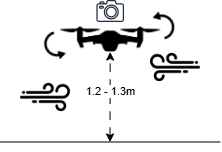
\includegraphics[width=0.4
    \textwidth]{img/intro-drone-gray4.PNG}
    \caption{Survelliance Drone Diagram}
\end{figure}

The proposed system architecture comprises a custom-designed \gls{pcb} flight controller integrating onboard power distribution, sensing, and control modules. Flight stabilisation and altitude maintenance are achieved through sensor fusion of inertial and distance measurements processed via integrated control algorithms. The design should incorporate safety features including shrouded propellers or propeller guards, low-battery auto-landing capability, and an emergency failsafe mechanism that initiates a controlled landing or motor shutdown following a communication loss exceeding thirty seconds. Moreover, the drone is constrained to operate on 1S or 2S lithium polymer batteries with a maximum capacity of 800 mAh and is required to sustain a minimum flight duration of three minutes. All components and materials must conform to the allocated project budget of AUD \$350. The overarching purpose of this design is to deliver a robust, safe, and open-source indoor drone platform that satisfies all operational, safety, and budgetary requirements. 

\subsection{Background}
\glspl{uav} combine sensing, computation, and actuation to achieve controlled flight through coordinated motor thrust. Their operation depends on precise feedback control systems that maintain stability and orientation while responding to pilot or autonomous commands. This is typically accomplished through onboard microcontrollers running real-time control algorithms that process data from inertial and range sensors to adjust motor outputs dynamically.

\begin{figure}[H]
    \centering
    \captionsetup{justification=centering, margin=1cm}
    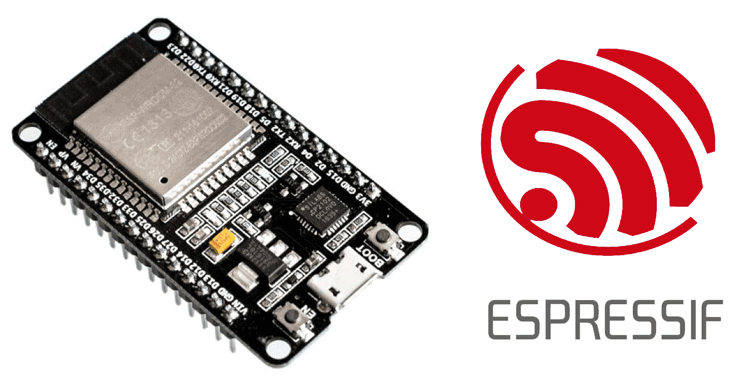
\includegraphics[width=0.42\textwidth]{img/intro-espressif.PNG}
    \caption{Espressif ESP32 DevKit~\cite{iotdesignpro2019}}
\end{figure}

The ESP32 microcontroller has emerged as a compact and cost-effective platform for such systems, integrating dual-core processing, Wi-Fi connectivity, and sufficient computational power to handle both flight control and communication tasks. Its compatibility with open-source development frameworks such as Espressif’s \gls{esp-idf} enables flexible low-level implementations of control loops, sensor fusion, and telemetry within a single embedded system.

In parallel, advances in printed circuit board (PCB) design allow the integration of flight electronics, power management, and motor drivers onto lightweight, custom boards that minimize wiring and improve reliability. 

\begin{figure}[H]
    \centering
    \captionsetup{justification=centering, margin=1cm}
    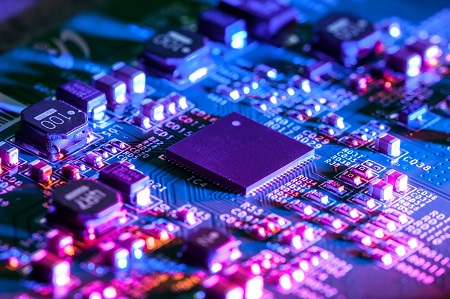
\includegraphics[width=0.4\textwidth]{img/intro-pcb.PNG}
    \caption{Printed Circuit Board \cite{mistral2020}}
\end{figure}

Together, these developments make it feasible to design small-scale, low-cost autonomous drones capable of stable flight and sensor-based navigation for educational, research, and experimental applications.

\subsection{Summary of Contributions}
\temp{To-do}

\subsection{Report Structure}
This report is structured to provide a comprehensive overview of the design and development of the autonomous ESP32-based drone. Section 1 introduces the project, outlining its scope, purpose, background, and key contributions. Section 2 details the design process, including system requirements, hardware and firmware architecture, component selection, and integration. It also addresses testing procedures, safety, ethical considerations, and identified risks. Section 3 presents recommendations for further development and improvement. Section 4 provides the user manual for operation and maintenance of the system, and Section 5 lists all referenced materials and supporting documentation. Any additional material can be found in the Appendices.


